\section{Global-view Communication and Synchronization Constructs}

\subsection{{\tt reflect} Construct} \label{sub:reflect}

\subsubsection*{Synopsis}
The {\tt \Directive{reflect}} construct assigns the value of a
reflection source to the corresponding shadow object.

\subsubsection*{Syntax}
\Syntax{reflect}
\begin{tabular}{ll}
 \verb![F]! & \verb|!$xmp| {\tt reflect} \verb|(| {\it array-name}
 {\openb}, {\it array-name}{\closeb}... \verb|)| {\bsquare} \\
 &\hspace{0.3cm} {\bsquare} {\openb}{\tt width (} {\it reflect-width}
     {\openb}, {\it reflect-width}{\closeb}... {\tt )}{\closeb}
     {\openb}{\tt orthogonal}{\closeb}
     {\openb}{\tt async (} {\it async-id} {\tt )}{\closeb} \\
\verb![C]! & \verb|#pragma xmp| {\tt reflect} \verb|(| {\it array-name}
     {\openb}, {\it array-name}{\closeb}... \verb|)| {\bsquare} \\
 &\hspace{0.3cm} {\bsquare} {\openb}{\tt width (} {\it reflect-width}
     {\openb}, {\it reflect-width}{\closeb}... {\tt )}{\closeb}
     {\openb}{\tt orthogonal}{\closeb}
     {\openb}{\tt async (} {\it async-id} {\tt )}{\closeb} \\
\end{tabular}

\vspace{0.3cm}

where {\it reflect-width} must be one of:

\vspace{0.3cm}

\begin{tabular}{ll}
 \hspace{0.5cm} & {\openb}{\tt /periodic/}{\closeb} {\it int-expr} \\
                & {\openb}{\tt /periodic/}{\closeb} {\it int-expr} : {\it int-expr}
\end{tabular}

\subsubsection*{Description}

The {\tt reflect} construct updates each of the shadow objects of the
array specified by {\it array-name} with the value of its corresponding
reflection source. Note that the shadow objects corresponding to
elements at the non-orthogonal positions are also updated with this
construct, unless the {\tt orthogonal} clause is specified.

%copies the value of the reflection source of
%the reflect-object specified by {\it array-name} to all shadow
%objects.
%This directive may execute the communications.

When the {\tt width} clause is specified and takes the form ``{\it
int-expr} : {\it int-expr}'' in a dimension, the shadow area having the
width specified by the first {\it int-expr} at the lower bound and that
specified by the second one at the upper bound in the dimension are
updated.
%
When the {\tt width} clause is specified, and takes the form {\it int-expr},
the shadow areas having the same width specified at both the upper
and lower bounds in the dimension are updated.
%
When the {\tt width} clause is omitted, the whole shadow area of the array
is updated.

In particular, when the \Term{{\tt /periodic/} modifier} is specified in
{\it reflect-width}, the update of the shadow object in the dimension is
``periodic,'' which means that the shadow object at the global lower
(upper) bound is treated as if it corresponds to the data object of the
global upper (lower) bound, and is updated with that value by the {\tt
reflect} construct.

When the {\tt orthogonal} clause is specified, only the shadow objects
corresponding to elements at the orthogonal positions are updated by the
{\tt reflect} construct.
%the shadow object is updated only by orthogonal nodes.

When the {\tt async} clause is specified, the statements following this
construct may be executed before the operation is complete.

\subsubsection*{Restrictions}

\begin{itemize}
 \item The arrays specified by the sequence of {\it array-names} must
       be mapped onto the executing node set.
 \item The reflect width of each dimension specified by the {\it
       reflect-width} must not exceed the shadow width of the arrays.
 \item The {\tt reflect} construct is global, which means that it must be
       executed by all nodes in the current executing node set, and each local
       variable referenced in the construct must have the same value
       among all of them.
 \item {\it async-id} must be an expression of type default integer in
       {\XMPF} or type {\tt int} in {\XMPC}.
\end{itemize}

\subsubsection*{Example}
\Example{reflect}
\Example{shadow}

\begin{XFexample}
!$xmp nodes p(4)
!$xmp template t(100)
!$xmp distribute t(block) onto p

      real a(100)
!$xmp align a(i) with t(i)
!$xmp shadow a(1)

      ...
!$xmp reflect (a) width (/periodic/1)
\end{XFexample}

\begin{myfigure}
\begin{center}
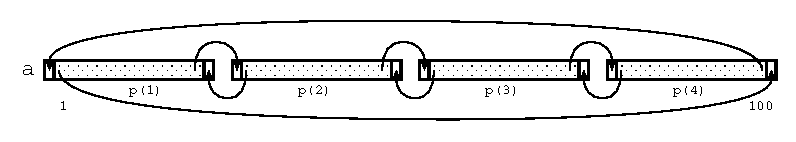
\includegraphics[width=0.9\hsize]{figs/fig3.2.eps}
\end{center}
\caption{Example of periodic shadow reflection.}
\label{fig3.2}
\end{myfigure}

The {\tt shadow} directive allocates ``periodic'' shadow areas of the
array {\tt a}.
The {\tt reflect} construct updates ``periodically'' the shadow area of
{\tt a} (Figure \ref{fig3.2}). A periodic shadow at the lower
bound on the node {\tt p(1)} is updated with the value of {\tt a(100)}
and that at the upper bound on {\tt p(4)} with the value of {\tt a(1)}.


\subsection{{\tt gmove} Construct}

\subsubsection*{Synopsis}

%The {\tt \Directive{gmove}} construct copies the data of a
%distributed array in the global view. 

The {\tt \Directive{gmove}} construct allows an assignment statement,
which may cause communication, to be executed possibly in parallel by
the executing nodes.

\subsubsection*{Syntax}
\Syntax{gmove}

\begin{tabular}{ll}
\verb![F]! & \verb|!$xmp| {\tt gmove} {\openb}{\tt in} $\vert$ {\tt
 out}{\closeb} {\openb}{\tt async (} {\it async-id} {\tt )}{\closeb}\\
% {\it dest} {\tt =} {\it source} \\
\verb![C]! & \verb|#pragma xmp| {\tt gmove} {\openb}{\tt in} $\vert$ {\tt
     out}{\closeb} {\openb}{\tt async (} {\it async-id} {\tt )}{\closeb}\\
% {\it dest} {\tt =} {\it source} \\
\end{tabular}

\subsubsection*{Description}

This construct copies the value of the right-hand side variable
into the left-hand side of the associated assignment statement,
which may cause communication between the executing nodes. Such
communication is detected, scheduled, and performed by the XcalableMP
runtime system.

%This construct executes a copy operation of the global data array object
%distributed into nodes.
%This directive is followed by the assignment
%statement of the scalar value and array sections.
%The assignment may require communication between nodes.

%Note that, in {\XMP}, the {\C} language is extended to support array
%section notation in order to support an assignment of array objects.

%The assignment statement must have one of the following patterns:
%
%\begin{itemize}
%\item  Scalar assignment. For example:
%
%\begin{tabular}{lll}
%\hspace{0.5cm} & {\tt s1 = s2} & ! {\tt s1} and {\tt s2} is a scalar
%variable \\ 
%& {\tt a(3) = b(i, j)} & ! {\tt a} and {\tt b} are arrays. \\
%\end{tabular}
%
%\item Array assignment. The left-hand-side variable must be either an
%      array name, an array section, or a scalar object. For example:
%
%\begin{tabular}{lll}
%\hspace{0.5cm} & {\tt a = b} & ! {\tt a} and {\tt b} are arrays \\
% & {\tt a(1:10) = b(n:n+9, k)} & ! left-hand side and right-hand side are array sections \\
% & {\tt a(1:10) = s2} & ! left-hand side is an array section and right-hand side is a
% scalar variable \\
% & {\tt a(1:10) = b(i, j)} & ! left-hand side is an array section and right-hand side is a
% scalar object \\
%\end{tabular}
%\end{itemize}

%The {\tt gmove} construct must be executed by all of the executing
%nodes. The value of scalar objects, the index value, and the range
%value of the array section in the assignment statement must be the same in
%every node executing this directive.

There are three operating modes of the {\tt gmove} construct:

\begin{itemize}
 \item {\bf collective mode}\index{collective mode (of {\tt gmove})}

       When neither the {\tt in} nor the {\tt out} clause is specified,
       the copy operation is performed collectively, and results in 
       implicit synchronization among the executing nodes.

       If the {\tt async} clause is not specified, then the construct is
       ``synchronous,'' and it is guaranteed that the left-hand side
       data can be read and overwritten, the right-hand side data can be
       overwritten, and all of 
       the operations of the construct on the executing nodes are
       completed when returning from the construct;
       otherwise, the construct is ``asynchronous,'' and it is not
       guaranteed that the operations are completed, until the
       associating {\tt wait\_async} construct (Section
       \ref{subsec:wait_async Construct}) is completed.

%In this case, all elements in both the source array and the target array
%must be distributed onto the executing node set.
%If the object on the right-hand side is a local
%object, then the value of the local object must be the same.
%
%In this case, the assignment is performed locally, where the object on
%the left-hand side is distributed.
%
%If the object on the left-hand side is a local object
%and the object on the right-hand side is global, then this operation
%performs broadcast operation.

 \item {\bf in mode}\index{in mode (of {\tt gmove})}

       When the {\tt in} clause is specified, the right-hand side data of the
       assignment, all or part of which may reside outside the
       executing node set, can be transferred from its owner nodes to
       the executing nodes by this construct.

       If the {\tt async} clause is not specified, then the construct is
       ``synchronous,'' and it is guaranteed that the left-hand side data
       can be read and overwritten, and that all of the operations of the
       construct on the owner nodes of the right-hand side and the executing nodes
       are completed when returning from the construct;
       otherwise, the construct is ``asynchronous,'' and it is not
       guaranteed that the operations are completed, until the
       associating {\tt wait\_async} construct (Section
       \ref{subsec:wait_async Construct}) is completed.

 \item {\bf out mode}\index{out mode (of {\tt gmove})}

       When the {\tt out} clause is specified, the left-hand side data of the
       assignment, all or part of which may reside outside the 
       executing node set, can be transferred from the executing nodes
       to its owner nodes by this construct.

       If the {\tt async} clause is not specified, then the construct is
       ``synchronous,'' and it is guaranteed that the right-hand side data
       can be overwritten, and that all of the operations of the construct on
       the owner nodes of the left-hand side and the executing nodes are
       completed when returning from the construct; otherwise, the
       construct is ``asynchronous,'' and it is not guaranteed that the
       operations are completed, until the associating {\tt wait\_async}
       construct (Section \ref{subsec:wait_async Construct}) is completed.

\end{itemize}

%Note that, in these cases, no synchronization is implied and it is not
%ensured that the copy operation is completed. Thus, if a synchronization
%between the executing nodes and the owner nodes is required, the
%programmer must specify it explicitly by using a {\tt barrier} construct
%or a pair of a {\tt post} and an {\tt wait} construct.

%When an {\tt in} clause is specified, then the node that owns the
%element of the object on the left-hand side obtains the data on the
%right-hand side by the remote copy (get) operation.
%Therefore, the object on the left-hand side must be distributed onto
%the executing node set.
%
%When an {\tt out} clause is specified, then the node that owns the element
%of the object on the right-hand side places the data on the left-hand
%side by the remote copy (put) operation.
%Therefore, the object on the
%right-hand side must be distributed onto the executing node set.

%If no option is specified, then the copy can be performed by two-side
%communication. In this case, the receiver side waits for the sender side,
%resulting in implicit synchronization. 

%If an {\tt in} or {\tt out} clause is specified, then the
%copy operation should be performed by one-side communication for remote
%memory access. Thus, no synchronization is implied. If
%synchronization between reader and writer is required, then the programmer
%must perform synchronization explicitly by a {\tt barrier} construct. If
%the reader and the writer do not belong to the same executing node set,
%then point-to-point synchronization by {\tt post-wait} directive can be used.

When the {\tt async} clause is specified, the statements following this
construct may be executed before the operation is complete.

\subsubsection*{Restrictions}

\begin{itemize}
 \item The {\tt gmove} construct must be followed by (i.e., associated
       with) a simple assignment statement that contains neither
       arithmetic operations nor function calls.
 \item The {\tt gmove} construct is global, which means that it must be
       executed by all nodes in the current executing node set, and each local
       variable referenced in the construct must have the same value.
 \item If the {\tt gmove} construct is in the {\it collective} mode, then
       all elements of the distributed arrays appearing on both the
       left-hand side and the right-hand side of the associated assignment
       statement must reside in the executing node set.
 \item If the {\tt gmove} construct is in the {\it in} mode, then
       all elements of the distributed array appearing on the left-hand side of the
       associated assignment statement must reside in the executing node
       set.
 \item If the {\tt gmove} construct is in the {\it out} mode, then
       all elements of the distributed array appearing on the right-hand side of the
       associated assignment statement must reside in the executing node
       set.
 \item {\it async-id} must be an expression of type default integer in
       {\XMPF} or type {\tt int} in {\XMPC}.
\end{itemize}

\subsubsection*{Examples}
\begin{description}
\item[Example 1: Array assignment]
\Example{gmove}

If the arrays on both the left-hand side and the right-hand side are distributed, then the copy
operation is performed using all-to-all 
communication. If the left-hand side is a replicated array, this copy
is performed using multi-cast communication. If the right-hand side is a
replicated array, then no communication is required.

\vspace{0.5cm}

\begin{minipage}{0.45\hsize}
\begin{center}
\begin{XFexample}
!$xmp gmove
      a(:,1:N) = b(:,3,0:N-1)
\end{XFexample}
\end{center}
\end{minipage}
\begin{minipage}{0.45\hsize}
\begin{center}
\begin{XCexampleR}
#pragma xmp gmove
      a[1:N][:] = b[0:N][3][:];
\end{XCexampleR}
\end{center}
\end{minipage}
\vspace{1cm}

\item[Example 2: Scalar assignment to an array] 

When the right-hand side is an element of a distributed array, the copy operation
is performed by broadcast communication from the owner of the element. If 
the right-hand side is a replicated array, then no communication is required.

\vspace{0.5cm}

\begin{minipage}{0.45\hsize}
\begin{center}
\begin{XFexample}
!$xmp gmove
      a(:,1:N) = c(k)
\end{XFexample}
\end{center}
\end{minipage}
\begin{minipage}{0.45\hsize}
\begin{center}
\begin{XCexampleR}
#pragma xmp gmove
      a[1:N][:] = c[k]
\end{XCexampleR}
\end{center}
\end{minipage}
\vspace{1cm}

\item[Example 3: in mode assignment]

	   Because {\tt b(3)} referenced on the right-hand side of the
	   {\tt gmove} construct does not reside in the executing node
	   set ({\tt p(1:2)}), the construct is executed in the {\it in}
	   mode. Thus, {\tt b(3)} is transferred from its owner node
	   {\tt p(3)} to the executing node set.

	   Until {\tt p(1:2)} returns from the
	   construct, there is no gurantee that any node can read and
	   overwrite {\tt a(1:2)},
	   and that any relevant operations on {\tt p(1:2)} and {\tt p(3)}
	   are completed.

\vspace{0.5cm}

\begin{XFexample}
!$xmp nodes p(4)
!$xmp template t(4)
!$xmp distribute t(block) onto p

      real a(4), b(4)
!$xmp align (i) with t(i) : a, b
      ...
!$xmp task on p(1:2)
      ...
!$xmp gmove in
      a(1:2) = b(2:3)
      ...
!$xmp end task
\end{XFexample}

%$

\end{description}

\subsection{{\tt barrier} Construct}

\subsubsection*{Synopsis}

The {\tt \Directive{barrier}} construct specifies an explicit barrier
at the point at which the construct appears. 

\subsubsection*{Syntax}
\Syntax{barrier}

\begin{tabular}{ll}
\verb![F]! & \verb|!$xmp| {\tt barrier} {\openb}{\tt on} {\it nodes-ref}
 $\vert${\it template-ref}{\closeb} \\
\verb![C]! & \verb|#pragma xmp| {\tt barrier} {\openb}{\tt on} {\it
     nodes-ref} $\vert$ {\it template-ref}{\closeb} \\
\end{tabular}

\subsubsection*{Description}

The barrier operation is performed among the node set specified by
the {\tt on} clause. If no {\tt on} clause is specified, then it is
assumed that the current executing node set is specified in it.

Note that an {\tt on} clause may represent multiple node sets. In such a
case, a barrier operation is performed in each node set.

%The barrier construct also has the function of ensuring that all of the
%remote copy operations that are invoked by gmove in/out constructs
%executed by the node set specified by the {\tt on} clause are finished.

\subsubsection*{Restriction}

\begin{itemize}
\item The node set specified by the {\tt on} clause must be a subset of the
      executing node set.  
\end{itemize}


\subsection{{\tt reduction} Construct}

\subsubsection*{Synopsis}

The {\tt \Directive{reduction}} construct performs a reduction
operation among nodes. 

\subsubsection*{Syntax}
\Syntax{reduction}

\begin{tabular}{ll}
\verb![F]! & \verb|!$xmp| {\tt reduction (} {\it reduction-kind} {\it
  :} {\it variable} {\openb}, {\it variable} {\closeb}... {\tt )}
 {\bsquare} \\
 & \hspace{6cm} {\bsquare} {\openb}{\tt on} {\it node-ref} $\vert$ {\it
     template-ref}{\closeb} {\openb}{\tt async (} {\it async-id} {\tt
     )}{\closeb} \\
\end{tabular}

\vspace{0.5cm}

where {\it reduction-kind} is one of:

\begin{tabular}{ll}
 \hspace{0.5cm} & {\tt +} \\
 & {\tt *} \\
% & {\tt -} \\
 & {\tt .and.} \\
 & {\tt .or.} \\
 & {\tt .eqv.} \\
 & {\tt .neqv.} \\
 & {\tt max} \\
 & {\tt min} \\
 & {\tt iand} \\
 & {\tt ior} \\
 & {\tt ieor} \\
\end{tabular}

\vspace{0.5cm}

\begin{tabular}{ll}
 \hspace{-\parindent}
 \verb![C]! & \verb|#pragma xmp| {\tt reduction (} {\it reduction-kind} {\it
  :} {\it variable} {\openb}, {\it variable} {\closeb}... {\tt )}
 {\bsquare} \\
 & \hspace{6cm} {\bsquare} {\openb}{\tt on} {\it node-ref} $\vert$ {\it
     template-ref}{\closeb} {\openb}{\tt async (} {\it async-id} {\tt
     )}{\closeb} \\
\end{tabular}

\vspace{0.5cm}

where {\it reduction-kind} is one of:

\begin{tabular}{ll}
 \hspace{0.5cm} & {\tt +} \\
 & {\tt *} \\
% & {\tt -} \\
 & {\verb|&|} \\
 & {\tt |} \\
 & {\verb|^|} \\
 & {\verb|&&|} \\
 & {\tt ||} \\
 & {\tt max} \\
 & {\tt min} \\
\end{tabular}

\subsubsection*{Description}

The {\tt reduction} construct performs a type of
% modified by Sakagami,H. 09/11/13                                            
reduction operation specified by {\it reduction-kind} for the specified
local variables among the node set specified by the {\tt on}
clause, and it sets the reduction results to the variables on each of the
nodes.
%
Note that some of the reduction operations, namely, {\tt FIRSTMAX}, {\tt
FIRSTMIN}, {\tt LASTMAX}, and {\tt LASTMIN}, which can be specified in
the {\tt reduction} clause of the {\tt loop} directive, cannot be
specified in the {\tt reduction} construct because their semantics are
not defined for it.
%
The variable specified by {\it variable}, which is the target of the
reduction operation, is referred to as the ``\Term{reduction
variable}.'' After the reduction operation, the value of a reduction
variable becomes the same in every node that performs the operation.

The reduction result is computed by combining the reduction variables on
all of the nodes using the reduction operator. The ordering of this
reduction is unspecified.

When the {\tt async} clause is specified, the statements following this
construct may be executed before the operation is complete.

% inserted by Sakagami,H. 09/11/13 ----- start ----                            
When {\it template-ref} is specified in the {\tt on} clause, the operation
is performed in a node set that consists of nodes onto which the
specified template section is distributed.
Therefore, before the {\tt reduction} construct is executed, the
referenced template must be fixed.
%
%When {\it template-subscript} in the {\it template-ref} is ``*'', nodes
%in the corresponding dimension are ignored for the reduction operation.
%
%When {\it template-subscript} in the {\it template-ref} is {\it
%triplet}, nodes for all template elements in the corresponding dimension
%perform the reduction operation.
%
When {\it nodes-ref} is specified in the {\tt on} clause, the operation
is performed in the specified node set.
%Therefore, before the {\tt \Directive{reduction}} construct is executed,
%the referenced node set must be fixed.
%
When the {\tt on} clause is omitted, the operation is performed in the
executing node set.

Note that an {\tt on} clause may represent multiple node sets. In such a
case, a reduction operation is performed in each node set.

\subsubsection*{Restrictions}

\begin{itemize}
%\item {\it template-spec} appearing in {\it template-ref} must be either ``*'', ``\
%:'' or the range.
%\item If {\tt on} clause is omitted, the operation is done in the current execu\
%ting node.
 \item The variables specified by the sequence of {\it variables} must
       either not be aligned or must be replicated among nodes of the node
       set specified by the {\tt on} clause.
 \item The {\tt reduction} construct is global, which means that it must
       be executed by all nodes in the current executing node set, and each local
       variable referenced in the construct must have the same value.
 \item {\it async-id} must be an expression of type default integer in
       {\XMPF} or type {\tt int} in {\XMPC}.
 \item The node set specified by the {\tt on} clause must be a subset of the
       executing node set.
\end{itemize}
% inserted by Sakagami,H. 09/11/13 ----- end ---- 

\subsubsection*{Examples}
\Example{reduction}

\begin{description}
\item[Example 1]
\hspace{\hsize}
\begin{XFexample}
!$xmp reduction(+:s)
!$xmp reduction(max:aa) on t(*,:)
!$xmp reduction(min:bb) on p(10:30)
\end{XFexample}

% modified by Sakagami,H. 09/11/13                                             
%In the first example, the scalar variable {\tt s} is assumed to contain the 
%partial sum of the variable, and the reduction operation calculates the
%total sum of the variable. The total sum is stored in the variable in
%each node.
In the first line, the reduction operation calculates the sum of the
scalar variable {\tt s} in the executing node set, and the result is
stored in the variable in each node.

% modified by Sakagami,H. 09/11/13                                             
The reduction operation in the second line computes the maximum value of
the variable {\tt aa} in each node set onto which each of the template
sections specified by {\tt t(*,:)} is distributed.
%that consists of nodes associated with the
%range of the second dimension of template {\tt t}.

% modified by Sakagami,H. 09/11/13                
In the third line, the minimum value of the variable {\tt bb} in the node 
set specified by {\tt p(10:30)} is calculated. This example is
equivalent to the following code using the {\tt task} construct.

\begin{XFexample}
!$xmp task on p(10:30)
!$xmp reduction(min:bb)
!$xmp end task
\end{XFexample}

\item[Example 2]
\hspace{\hsize}
\begin{XFexample}
      dimension a(n,n), p(n), w(n)
!$xmp align a(i,j) with t(i,j)
!$xmp align p(i) with t(i,*)
!$xmp align w(j) with t(*,j)
      ...
!$xmp loop (j) on t(:,j)
      do j = 1, n
          sum = 0
!$xmp loop (i) on t(i,j) reduction(+:sum)
          do i = 1, n
              sum = sum + a(i,j) * p(i)
          end do
          w(j) = sum
      end do
\end{XFexample}

This code computes the matrix vector product,
% modified by Sakagami,H. 09/11/13
where a {\tt reduction} clause is specified for the {\tt \Directive{loop}}
construct of the inner loop. This is equivalent to the following code
snippet. 

\begin{XFexample}
!$xmp loop (j) on t(:,j)
      do j = 1, n
          sum = 0
!$xmp loop (i) on t(i,j) 
          do i = 1, n
              sum = sum + a(i,j) * p(i)
          end do
!$xmp reduction(+:sum) on t(1:n,j)
          w(j) = sum
      end do
\end{XFexample}

In these cases, the reduction operation on the scalar variable {\tt sum}
is performed for every iteration in the outer loop, which may cause a
large overhead.
% modified by Sakagami,H. 09/11/13
To reduce this overhead, the {\tt reduction} clause should be specified
in the {\tt \Directive{loop}} construct for the outer loop.
%
%because the loop index of the outer loop ({\tt j}) is different from that 
%for the reduction operation ({\tt i}).
This is because the node set in which the reduction operation is
performed is determined on the basis of its {\tt on} clause (see
\ref{sub:loop_construct}), and the {\tt on} clause of the outer {\tt
loop} construct is different from that of the inner one. 
%
However, this code can be modified using the {\tt reduction}
construct as follows: 

\begin{XFexample}
      dimension a(n,n), p(n), w(n)
!$xmp align a(i,j) with t(i,j)
!$xmp align p(i) with t(i,*)
!$xmp align w(j) with t(*,j)
      ...
!$xmp loop (j) on t(:,j)
      do j = 1, n
          sum = 0
!$xmp loop (i) on t(i,j) 
          do i = 1, n
              sum = sum + a(i,j) * p(i)
          end do
          w(j) = sum
      end do
!$xmp reduction(+:w) on t(1:n,*)
\end{XFexample}

This code performs a reduction operation on the array {\tt w} only once,
which may result in faster operation.  

\end{description}


\subsection{{\tt bcast} Construct}

\subsubsection*{Synopsis}

The {\tt \Directive{bcast}} construct performs broadcast communication
from a specified node.

\subsubsection*{Syntax}
\Syntax{bcast}

\begin{tabular}{ll}
 \verb![F]! & \verb|!$xmp| {\tt bcast} \verb|(| {\it variable} 
 {\openb}, {\it variable}{\closeb}... \verb|)|
 {\openb}{\tt from} {\it nodes-ref} $\vert$ {\it template-ref}{\closeb}
 {\bsquare} \\
 & \hspace{5cm} {\bsquare} {\openb}{\tt on} {\it nodes-ref}{\closeb}
     $\vert$ {\it template-ref}{\closeb}
     {\openb}{\tt async (} {\it async-id} {\tt )}{\closeb} \\

 \verb![C]! & \verb|#pragma xmp| {\tt bcast} \verb|(| {\it variable} 
 {\openb}, {\it variable}{\closeb}... \verb|)|
 {\openb}{\tt from} {\it nodes-ref}  $\vert$ {\it
     template-ref}{\closeb} {\bsquare} \\
 & \hspace{5cm} {\bsquare} {\openb}{\tt on} {\it nodes-ref} $\vert$ {\it
     template-ref}{\closeb}
 {\openb}{\tt async (} {\it async-id} {\tt )}{\closeb} \\

\end{tabular}

\subsubsection*{Description}

The values of the variables specified by the sequence of {\it
variables} (called {\it \Term{broadcast variables}}) are broadcasted 
from the node specified by the {\tt from} clause (called the
{\it \Term{source node}}) to each of the nodes in the node set specified
by the {\tt on} clause. After executing this construct,
the values of the broadcast variables become the same as those in the
source node.
%
If the {\tt from} clause is omitted, then the {\it first}
node, that is, the leading one in Fortran's array element order, of the
node set specified by the {\tt on} clause is assumed to be a source
node.
%
If the {\tt on} clause is omitted, then it is assumed that the current
executing node set is specified in it.

When the {\tt async} clause is specified, the statements following this
construct may be executed before the operation is complete.

\subsubsection*{Restrictions}

\begin{itemize}
 \item The variables specified by the sequence of {\it variables} must
       either not be aligned or must be replicated among nodes of the node set
       specified by the {\tt on} clause.
 \item The {\tt bcast} construct is global, which means that it must be
       executed by all nodes in the current executing node set, and each local
       variable referenced in the construct must have the same value
       among all of them.
 \item {\it async-id} must be an expression of type default integer in
       {\XMPF} or type {\tt int} in {\XMPC}.
 \item The node set specified by the {\tt on} clause must be a subset of
       the executing node set.
 \item The source node specified by the {\tt from} clause must belong to
       the node set specified by the {\tt on} clause.
 \item The source node specified by the {\tt from} clause must be one node.
\end{itemize}


\subsection{{\tt wait\_async} Construct}
\label{subsec:wait_async Construct}

\subsubsection*{Synopsis}

The {\tt \Directive{wait\_async}} construct guarantees that asynchronous
communications specified by {\it async-id} are complete.

\subsubsection*{Syntax}
\Syntax{wait\_async}

\begin{tabular}{ll}
\verb![F]! & \verb|!$xmp| {\tt wait\_async ( {\it async-id} {\openb},
 {\it async-id} {\closeb}... )} {\openb}{\tt on} {\it nodes-ref} $\vert$
 {\it template-ref}{\closeb} \\
\verb![C]! & \verb|#pragma xmp| {\tt wait\_async ( {\it async-id} {\openb},
 {\it async-id} {\closeb}... )} {\openb}{\tt on} {\it nodes-ref} $\vert$
 {\it template-ref}{\closeb}\\
\end{tabular}

\subsubsection*{Description}

The {\tt \Directive{wait\_async}} construct will block, and therefore
statements following it will not be executed, until the completion of
all of 
the asynchronous communications that are specified by {\it async-id}'s
and issued on the node set specified by the {\tt on} clause.
\mytextcolor{red}{
If an {\it async-id} is not associated with any asynchronous
communication, the {\tt wait\_async} construct ignores it.
}

\subsubsection*{Restrictions}

\begin{itemize}
 \item {\it async-id} must be an expression of type default integer in
       {\XMPF} or type {\tt int} in {\XMPC}.
 \item \mytextcolor{red}{\sout{{\it async-id} must be associated with an asynchronous
       communication using the {\tt async} clause of a communication
       construct.}}
 \item The {\tt wait\_async} construct is global, which means that it must
       be executed by all nodes in the current executing node set, and
       each local variable referenced in the construct must have the
       same value among all of them.
 \item The node set specified by the {\tt on} clause must be the same as
       those of the global constructs that initiate the asynchronous
       communications specified by {\it async-id}.
%\item Every communication specified by each {\it async-id} must be
%      executed on the same executing node set.
\end{itemize}


\subsection{{\tt async} Clause}
\index{async clause@{\tt async} clause}
\index{Directive!async clause@{{\tt async} clause}}

\subsubsection*{Synopsis}

The {\tt async} clause of the {\tt reflect}, {\tt gmove}, {\tt
reduction}, and {\tt bcast} constructs enables the corresponding
communication to be performed asynchronously.

\subsubsection*{Description}

Communication corresponding to the construct with an {\tt async} clause
is performed asynchronously, that is, it is initiated but not completed,
and therefore, statements following it may be executed before the
communication is complete.

%\subsubsection*{Restrictions}
%
%\begin{itemize}
% \item A node must not issue at runtime an asynchronous communication
%       with an {\tt async-id} until every other one with the same {\tt
%       async-id} is complete.
%\end{itemize}

\subsubsection*{Example}
\Example{async}
\Example{wait\_async}

\begin{XFexample}
!$xmp reflect (a) async(1)
      S1
!$xmp wait_async(1)
      S2
\end{XFexample}

The {\tt reflect} construct on the first line matches the {\tt wait}
construct on the third line because both of their {\it async\_id}
evaluate to one.
%
These constructs ensure that statements in {\tt S1} can be executed
before the {\tt reflect} communication is complete, and no statement in
{\tt S2} is executed until the {\tt reflect} communication is
complete.


\mytextcolor{red}{
\subsection{{\tt reduce\_shadow} Construct}
\label{154624_16Jan17}
}

\subsubsection*{Synopsis}

The {\tt \Directive{reduce\_shadow}} construct adds values of shadow
objects to their reflection source.

\subsubsection*{Syntax}
\Syntax{reduce\_shadow}

\begin{tabular}{ll}
 \verb![F]! & \verb|!$xmp| {\tt reduce\_shadow} \verb|(| {\it array-name}
 {\openb}, {\it array-name}{\closeb}... \verb|)| {\bsquare} \\
 &\hspace{0.3cm} {\bsquare} {\openb}{\tt width (} {\it reflect-width}
     {\openb}, {\it reflect-width}{\closeb}... {\tt )}{\closeb}
     {\openb}{\tt orthogonal}{\closeb}
     {\openb}{\tt async (} {\it async-id} {\tt )}{\closeb} \\
\verb![C]! & \verb|#pragma xmp| {\tt reduce\_shadow} \verb|(| {\it array-name}
     {\openb}, {\it array-name}{\closeb}... \verb|)| {\bsquare} \\
 &\hspace{0.3cm} {\bsquare} {\openb}{\tt width (} {\it reflect-width}
     {\openb}, {\it reflect-width}{\closeb}... {\tt )}{\closeb}
     {\openb}{\tt orthogonal}{\closeb}
     {\openb}{\tt async (} {\it async-id} {\tt )}{\closeb} \\
\end{tabular}

\subsubsection*{Description}

The {\tt reduce\_shadow} construct adds values of shadow objects of the
array specified by {\it array-name} to their reflection source. Note
that the shadow objects corresponding to elements at the non-orthogonal
positions are also added as the default behavior.

When the {\tt width} clause is specified and has the form ``{\it
int-expr} : {\it int-expr}'' in a dimension, the shadow areas having the
width specified by the first {\it int-expr} at the lower bound, and that
specified by the second one at the upper bound in the dimension are
added.
%
When the {\tt width} clause is specified and has the form {\it int-expr},
the shadow areas having the same width specified at both the upper
and lower bounds in the dimension are added.
%
When the {\tt width} clause is omitted, the whole shadow area of the array
is added.

In particular, when the \Term{{\tt /periodic/} modifier} is specified in
{\it reflect-width}, the addition of the shadow object in the dimension is
``periodic,'' which means that the shadow object at the global lower
(upper) bound is treated as if it corresponds to the data object of the
global upper (lower) bound and is added by the {\tt reduce\_shadow}
construct.

When the {\tt orthogonal} clause is specified,
the shadow object is added only by orthogonal nodes.

When the {\tt async} clause is specified, the statements following this
construct may be executed before the operation is complete.

\subsubsection*{Restrictions}

\begin{itemize}
 \item The arrays specified by the sequence of {\it array-names} must
       be mapped onto the executing node set.
 \item The width of each dimension specified by {\it
       reflect-width} must not exceed the shadow width of the arrays.
 \item The {\tt reduce\_shadow} construct is global, which means that it must be
       executed by all nodes in the current executing node set, and each local
       variable referenced in the construct must have the same value
       among all of them.
 \item {\it async-id} must be an expression of type default integer in
       {\XMPF} or type {\tt int} in {\XMPC}.
\end{itemize}

\subsubsection*{Examples}
\Example{reduce\_shadow}

\begin{XFexample}
      real rho(n,n)
!$xmp align rho(i,j) with t1(i,j)
!$xmp shadow rho(1:1)

      real f(m)
      integer x(m), y(m)
!$xmp align (k) with t2(k) : f, x, y

!$xmp loop on t2(k)
      do i = 1, no
        ix = x(i)
        iy = y(i)
        dx = x(i) - ix
        dy = y(i) - iy
        rho(ix  ,iy  ) = rho(ix  ,iy  ) + (1.0-dx)*(1.0-dy)*f(i)
        rho(ix+1,iy  ) = rho(ix+1,iy  ) +      dx *(1.0-dy)*f(i)
        rho(ix  ,iy+1) = rho(ix  ,iy+1) + (1.0-dx)*     dy *f(i)
        rho(ix+1,iy+1) = rho(ix+1,iy+1) +      dx *     dy *f(i)
      end do

!$xmp reduce_shadow (rho)
!$xmp reflect (rho)
\end{XFexample}

Assume that a two-dimensional field {\tt rho} and m particles are
both distributed onto nodes. On each node, a contribution of a particle
{\tt f(k)} is added to the nearest grid point of the field and its
neighbors, which may be in the shadow area on the node. In the last two
lines, the values of the shadow area from neighboring nodes are added to
the corresponding data object, and the results are then copied back to
the shadow area on the neighboring nodes.
